% 
%  chapter4.tex
%
\chapter{Architecture}\label{ch:architecture}
In this chapter we take a look at the architecture developed in the scope of CASCIFFO.
The chapter is structured as follows:
\begin{itemize}
    \item Global architecture~\ref{ch:architecture:sec:global-arch} - describes the global architecture used;
    \item Data Model~\ref{ch:architecture:sec:data-model} - presents the conceptual representation of the data structures that the application uses, and it defines how data is organized and related within the application.
\end{itemize}


\section{Global architecture}\label{ch:architecture:sec:global-arch}
The initial approach taken towards CASCIFFO was made following the monolithic architecture. A monolithic architecture consists in the development of software components within a single codebase. From an operating system's point of view, these components operate within one single application. The advantages brought by this design are centered around simplicity, the application is easier to deploy, test, debug and monitor. 
Applying this concept into context, the components developed were divided into three layers, the \acrshort{ui}, domain and data access layer. The first layer - data access layer - contains the data created and manipulated by the platform CASCIFFO; the second layer - domain layer - responsible for security and business processes within the platform; lastly the \acrshort{ui} layer corresponds to the presentation and logic of the user interface where user interaction begins.

The \acrlong{be} and \acrlong{fe} modules have distinct responsibilities within these layers, while the \acrshort{fe} contains all of the \acrshort{ui} layer, the \acrshort{be} consists of both domain and data access layer, as illustrated by~\ref{fig:layer-arch}. Finally, in addition to these layers, there's also a component inherent, although external, to the data access layer, the data base component, which is where all the data is stored.

\begin{figure}[H]
    \centering
    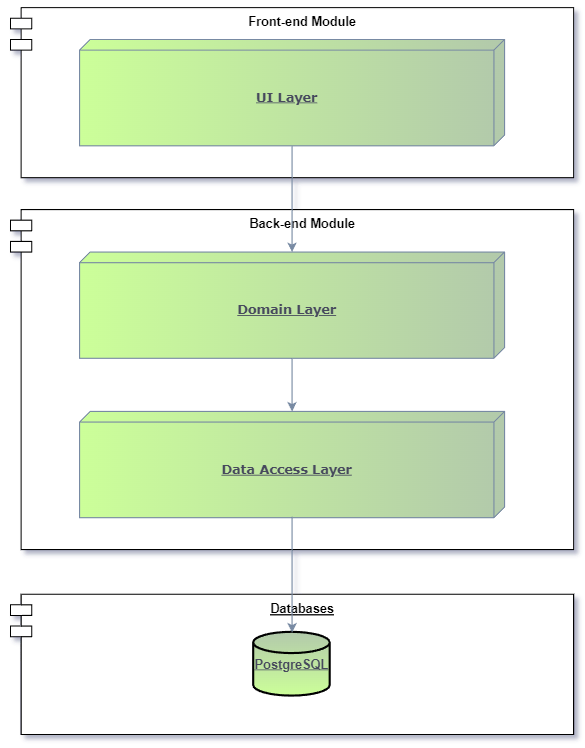
\includegraphics[scale=0.3]{Chapters/img/architecture/arch-layers.png}
    \caption{Layer Architecture}
    \label{fig:layer-arch}
\end{figure}

One of the drawbacks of this architecture is scalability and maintenance; the need of redeploying the entire application when a change is made, for example, a change in the \acrlong{fe} module should not imply an redeployment of the \acrlong{be} module as well. 
In wake of this, since we want a scalable solution, the layer based architecture was maintained while the monolithic aspect of a single codebase was discarded.
The modules were separated, allowing the \acrlong{fe} module and \acrlong{be} module to run independently of each other. Following the segregation of the modules, we also achieve independent deployments.

\subsection{Back-End module}
The \acrshort{be} module consists of the business logic and database access layers. The architecture used follows the Controller - Service - Repository pattern, frequently used in Spring Boot applications, as illustrated in figure~\ref{fig:domain-arch}. This pattern consists in having the controllers that manage REST requests and delegate business logic operations to a Service and after having processed the request, an appropriate response shall be created accordingly. 

\begin{figure}[H]
    \centering
    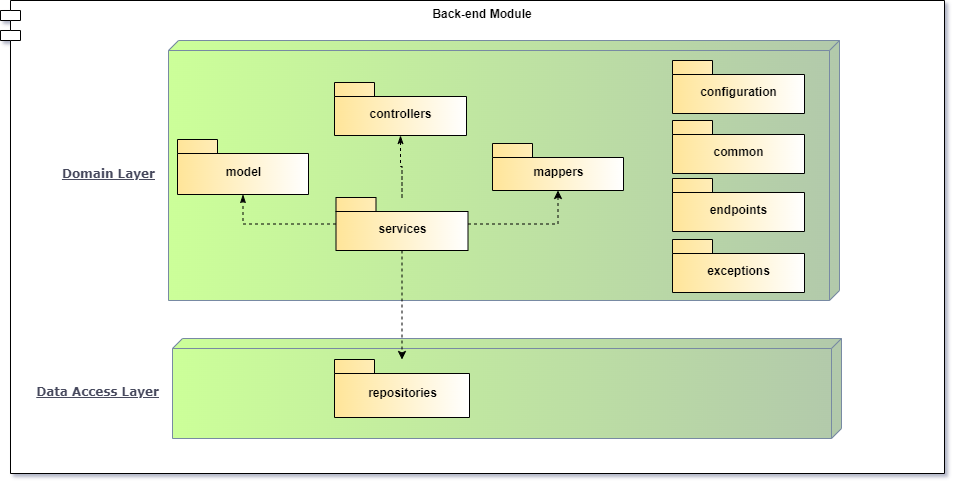
\includegraphics[scale=0.4]{Chapters/img/architecture/domain-dal-arch.drawio.png}
    \caption{Back-end module global architecture.}
    \label{fig:domain-arch}
\end{figure}

\subsection{Front-End module}
The \acrshort{fe} module consists of the \acrshort{ui} layer. The architecture, as viewed in figure~\ref{fig:ui-arch}, follows the same principle as the \acrshort{be} module, however, this time having designated Views for each page, each view utilizes a Service for data retrieval and both manipulate Model data. The Services are a stateless abstraction of the domain layer linked to their respective data model.

\begin{figure}[H]
    \centering
    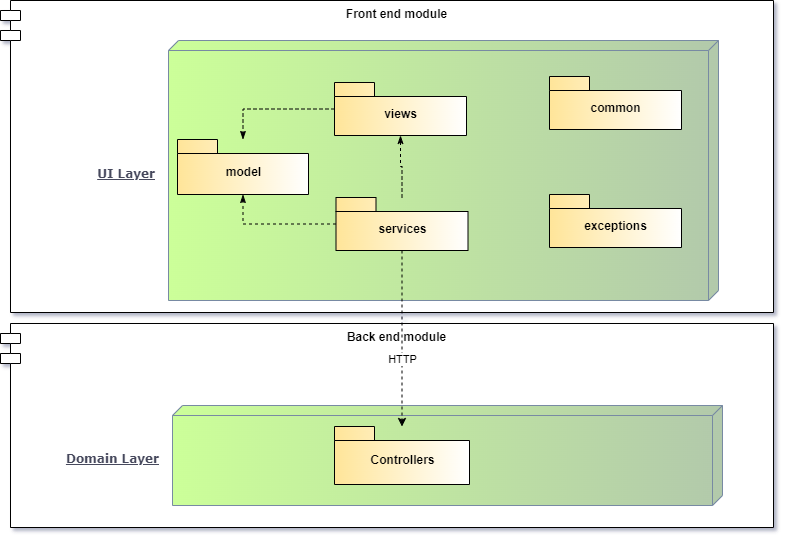
\includegraphics[scale=0.5]{Chapters/img/architecture/ui-domain-arch.png}
    \caption{Front-end module global architecture.}
    \label{fig:ui-arch}
\end{figure}


\section{Data model}~\label{ch:architecture:sec:data-model}

The data model created to satisfy the needs of the platform CASCIFFO was made while having an important limitation of the \textit{R2DBC} driver, originated from Spring Data JBDC, which only allows entities to have an numeric auto generated primary key, not permitting any composite keys, mentioned in the github issue "Add support for composite Id's"~\footnote{https://github.com/spring-projects/spring-data-r2dbc/issues/158}\label{fn:gh-issue-sd-r2dbc} which depends on the issue "Support for Composite Key via @Embeded plus @Id [DATAJDBC-352]"~\footnote{https://github.com/spring-projects/spring-data-relational/issues/574\#issue-776914525}\label{fn:gh-issue-sd-relations}. 

The model is is centered around two main entities, the first being the \lstinline{Proposal} entity which contains information regarding the submission and progress of a proposal of a clinical investigation. Secondly the \lstinline{Clinical Research} entity which contains information pertaining to a clinical trial or clinical observation that has had its proposal submitted, accepted and validated.

A \lstinline{Proposal} or \lstinline{Clinical Research} entity can refer to either a clinical trial or observation study, depending on the field \lstinline{research_type}. Although a clinical trial and an observational study are different, the information held by both is identical, differentiating only on existence of a financial component inherent to clinical trials. Therefore, these investigations can be stored regardless of their type in the mentioned entities. Aside from the identical data, another reason for choosing only one entity for representing clinical trials and observational studies in each stage, proposal submission and the active stage, is the amount of data stored, which is expected to be hundreds, so it makes it easier to do queries aimed at analyzing statistics.

This section is structured as such:
\begin{itemize}
    \item Users, Roles and States - Explains the user, roles and states entities as well as their own relationship;
    \item Proposal Entity - A detailed approach to the proposal entity and the entities surrounding it;
    \item Research Entity - A detailed approach to the research entity and the entities surrounding it.
\end{itemize}


\subsection{Users, Roles and States}
The proposal, clinical research and addenda entity require state to track their evolution over time, thus the \lstinline{State} entity was created, this entity holds all possible states for any proposal, clinical investigation or addenda. To differentiate between them an entity was created with the goal of interconnecting state chains. A state chain describes the flow from an initial state to a terminal state, i.e in the context of a proposal advancing from the state "Submetido" to "Validado". This entity, called, \lstinline[keywordstyle=\color{black},commentstyle=\color{black},stringstyle=\color{black}]{Next Possible States}, represents the possible transitions from one state to another, it contains two important fields that describe the chain the current state transition - \lstinline{state_type} - belongs to (i.e proposal, research or addenda), as well as the general order of the transition in the chain, initial for the first possible transition, progress for any in-between and terminal indicating the end of the chain.
To record the transitions, the entity State Transition was created, recording the previous state, new state, the date of transition, the type of transition (proposal, research or addenda) and finally the associated reference to what transitioned state. This reference is not a foreign key by choice, since it facilitates recording transitions in one entity rather than three different tables specifying the foreign relationship. 

As specified in the functional requirements, to advance states, a user requires a certain role associated to the state. This is represented through the entity \lstinline{State Roles}, which associates the entity states with the roles entity. In addition, the data model was created so that a user can have more than one role, hence the relationship entity \lstinline{User Roles}.
These entities can be viewed in figure~\ref{fig:er-diagram-users-roles-states}.


\begin{figure}[H]
    \centering
    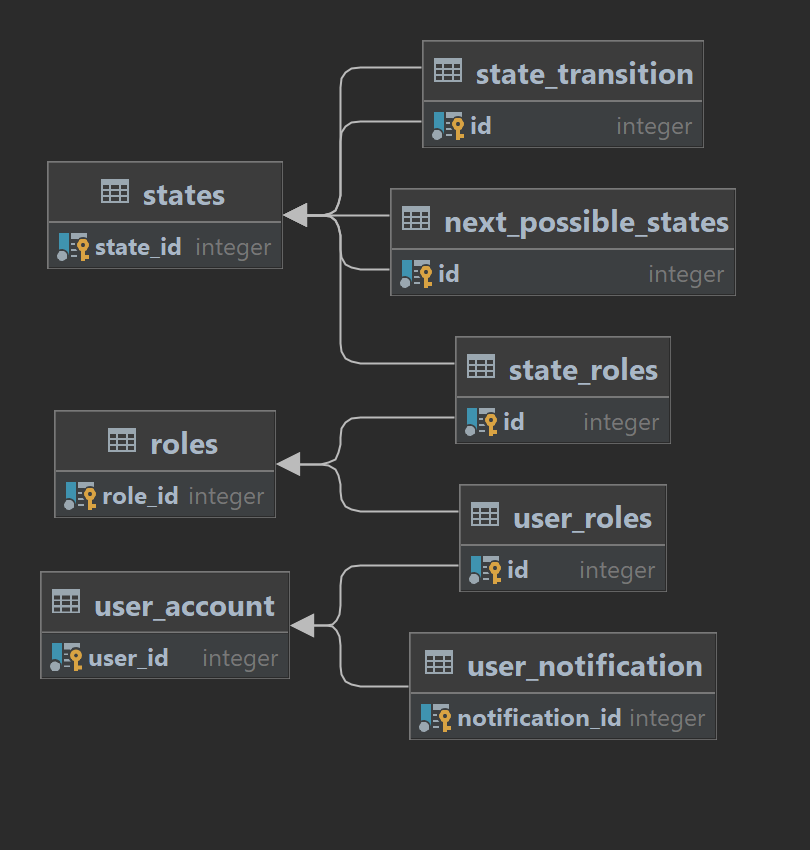
\includegraphics[scale=0.3]{Chapters/img/model/states-and-user-roles-er-diagram.png}
    \caption{Entity relationship diagram of users, roles and states.}
    \label{fig:er-diagram-users-roles-states}
\end{figure}

\subsection{Proposal Entity}
Associated to a proposal entity is the type of service it's included in, the therapeutic area and type of pathology, these three fields correspond to a foreign key to their own entities. Each of these entities consist of two fields, an \lstinline{identifier} and a \lstinline{name}. They were made into entities rather than simple fields to allow for consistency in the data model. This approach makes use of built-in foreign-key validations, which facilitates maintenance and CRUD operations on the entities. In addition to these fields, the proposal entity also includes a principal investigator responsible for submitting the proposal, an investigation team with all the investigators that can edit the proposal, a set of proposal comments made within the scope of the proposal, a financial component in case its a proposal for a clinical trial, a set of timeline events, the files associated to the proposal and most importantly the state, which corresponds to its current state. 

In addition to the need of tracking state, a proposal can have multiple file resources.
These files are stored on the operating system of the back-end module to avoid bloating the database with files. The information stored within the database through the entity \lstinline{Files} is the full-path, file size and name.

The diagram involving the entities centered around the proposal entity can be viewed in figure~\ref{fig:er-diagram-proposal}

\begin{figure}[H]
    \centering
    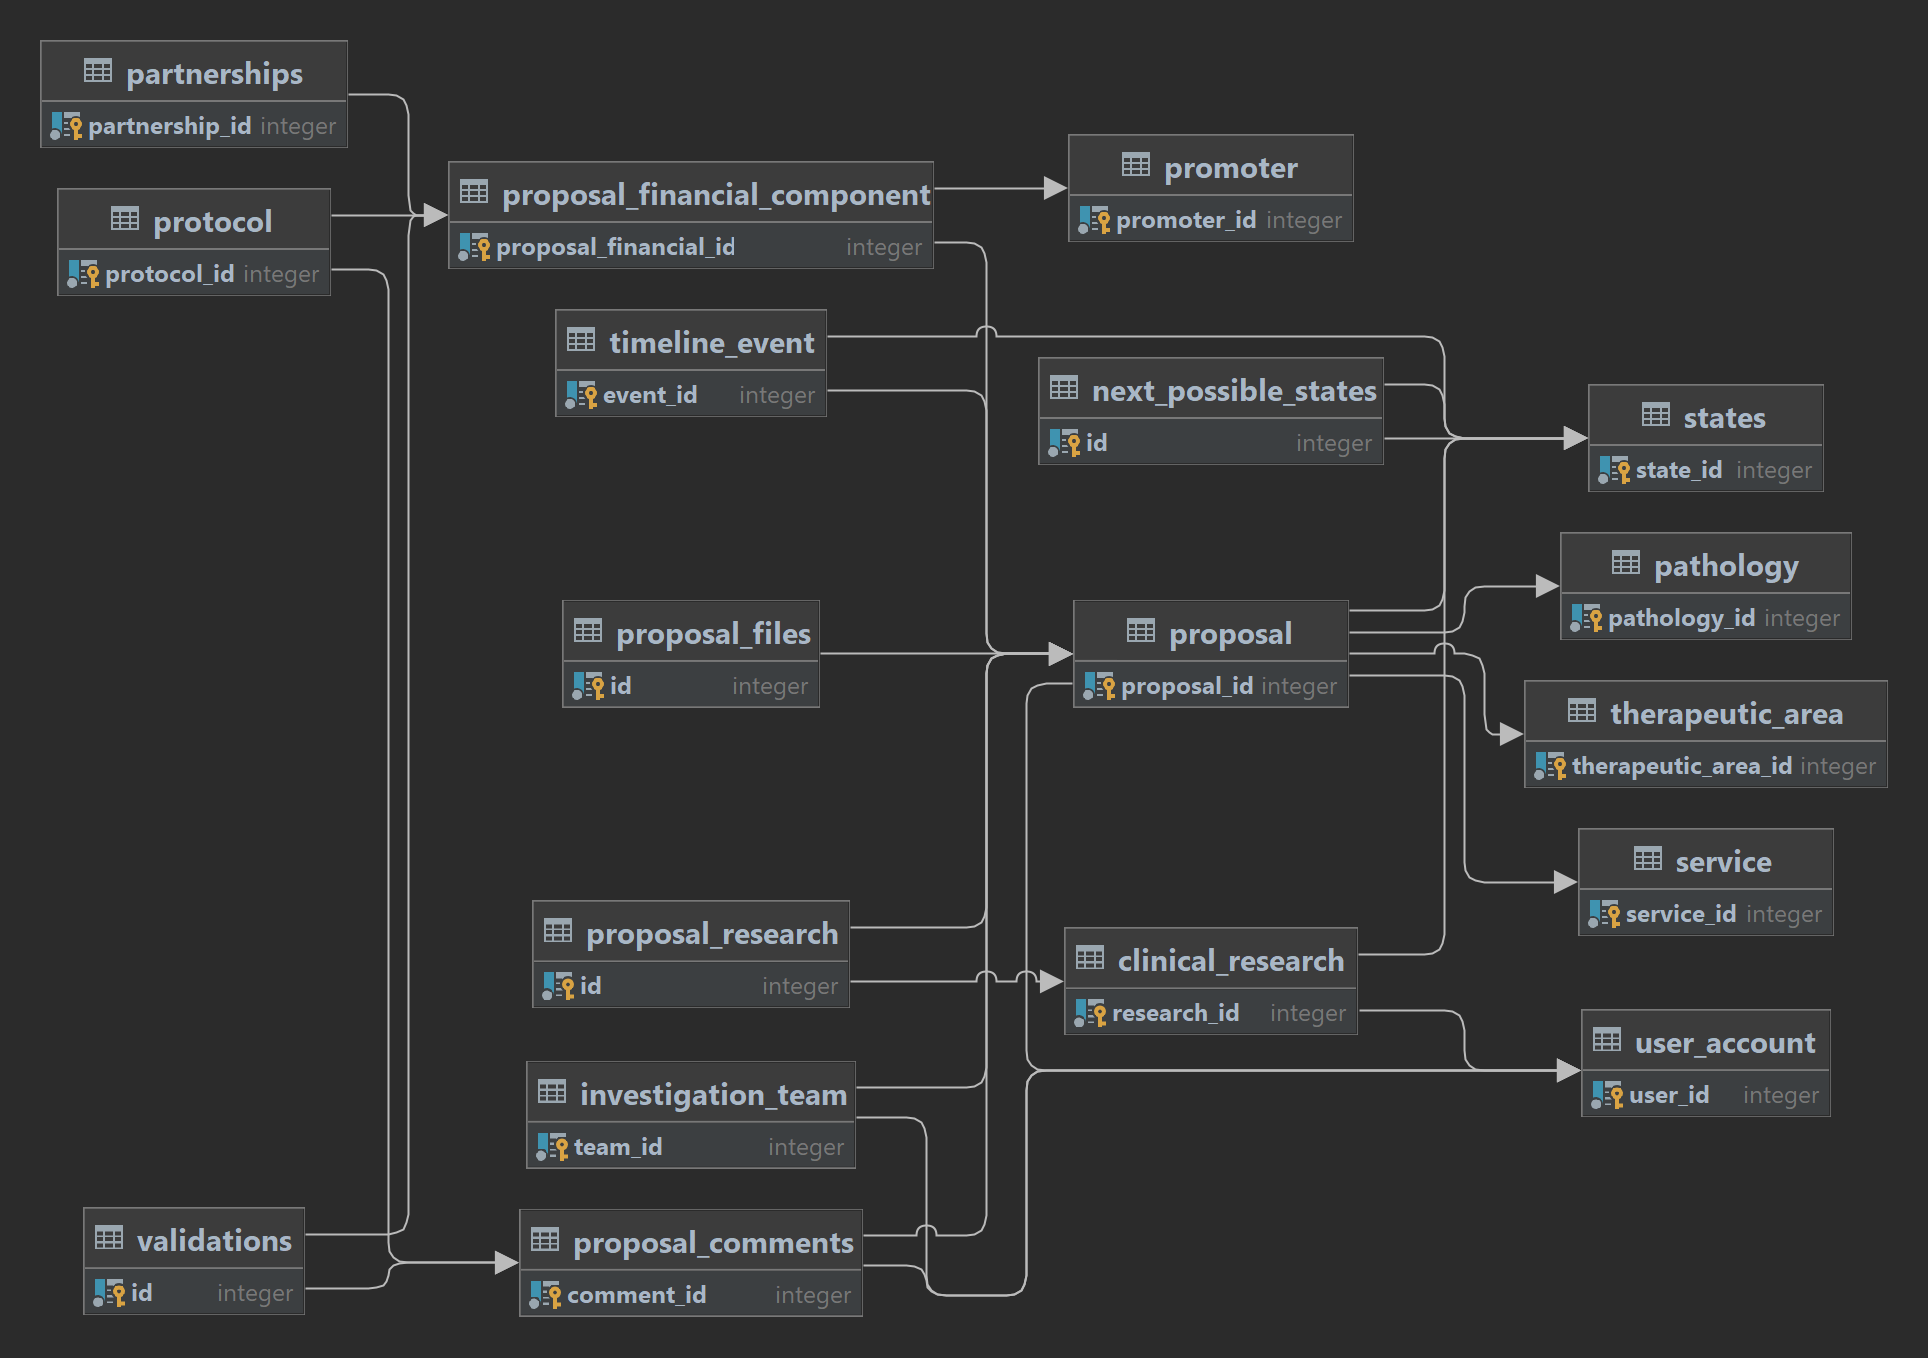
\includegraphics[scale=0.15]{Chapters/img/model/Proposal-centered-er-diagram.png}
    \caption{Entity relationship diagram centered on the Proposal Entity.}
    \label{fig:er-diagram-proposal}
\end{figure}

\subsection{Clinical Research}
A clinical research entity represents a clinical trial or observational trial and is associated to its proposal through the \lstinline{Proposal Research} entity which stores the association of each proposal to its clinical trial. A clinical research, in similarity to a proposal, also has a state to track its current status. In addition to this, it also has a list of visits that occur in the context of the investigation, a list of several addenda, a team of investigators, equal to the team submitted during its proposal stage and in case its a clinical trial it also has a financial component associated to it. It is to note that the financial component associated to a clinical research is different than a proposal's financial component. 

The research financial component is divided into two different sub categories, the team finance, which discriminates the revenue made by each team member and the clinical research finance, which represents the financial transactions made within the scope of the clinical research itself.

The addenda entity, associated to a clinical research, can have a file associated to it pertaining to the change being made, a state since it must undergo a validation process before it has an affect on the clinical research and a list of comments.

The diagram involving these entities centered around the clinical research entity can be viewed in figure~\ref{fig:er-diagram-research}.


\begin{figure}[H]
    \centering
    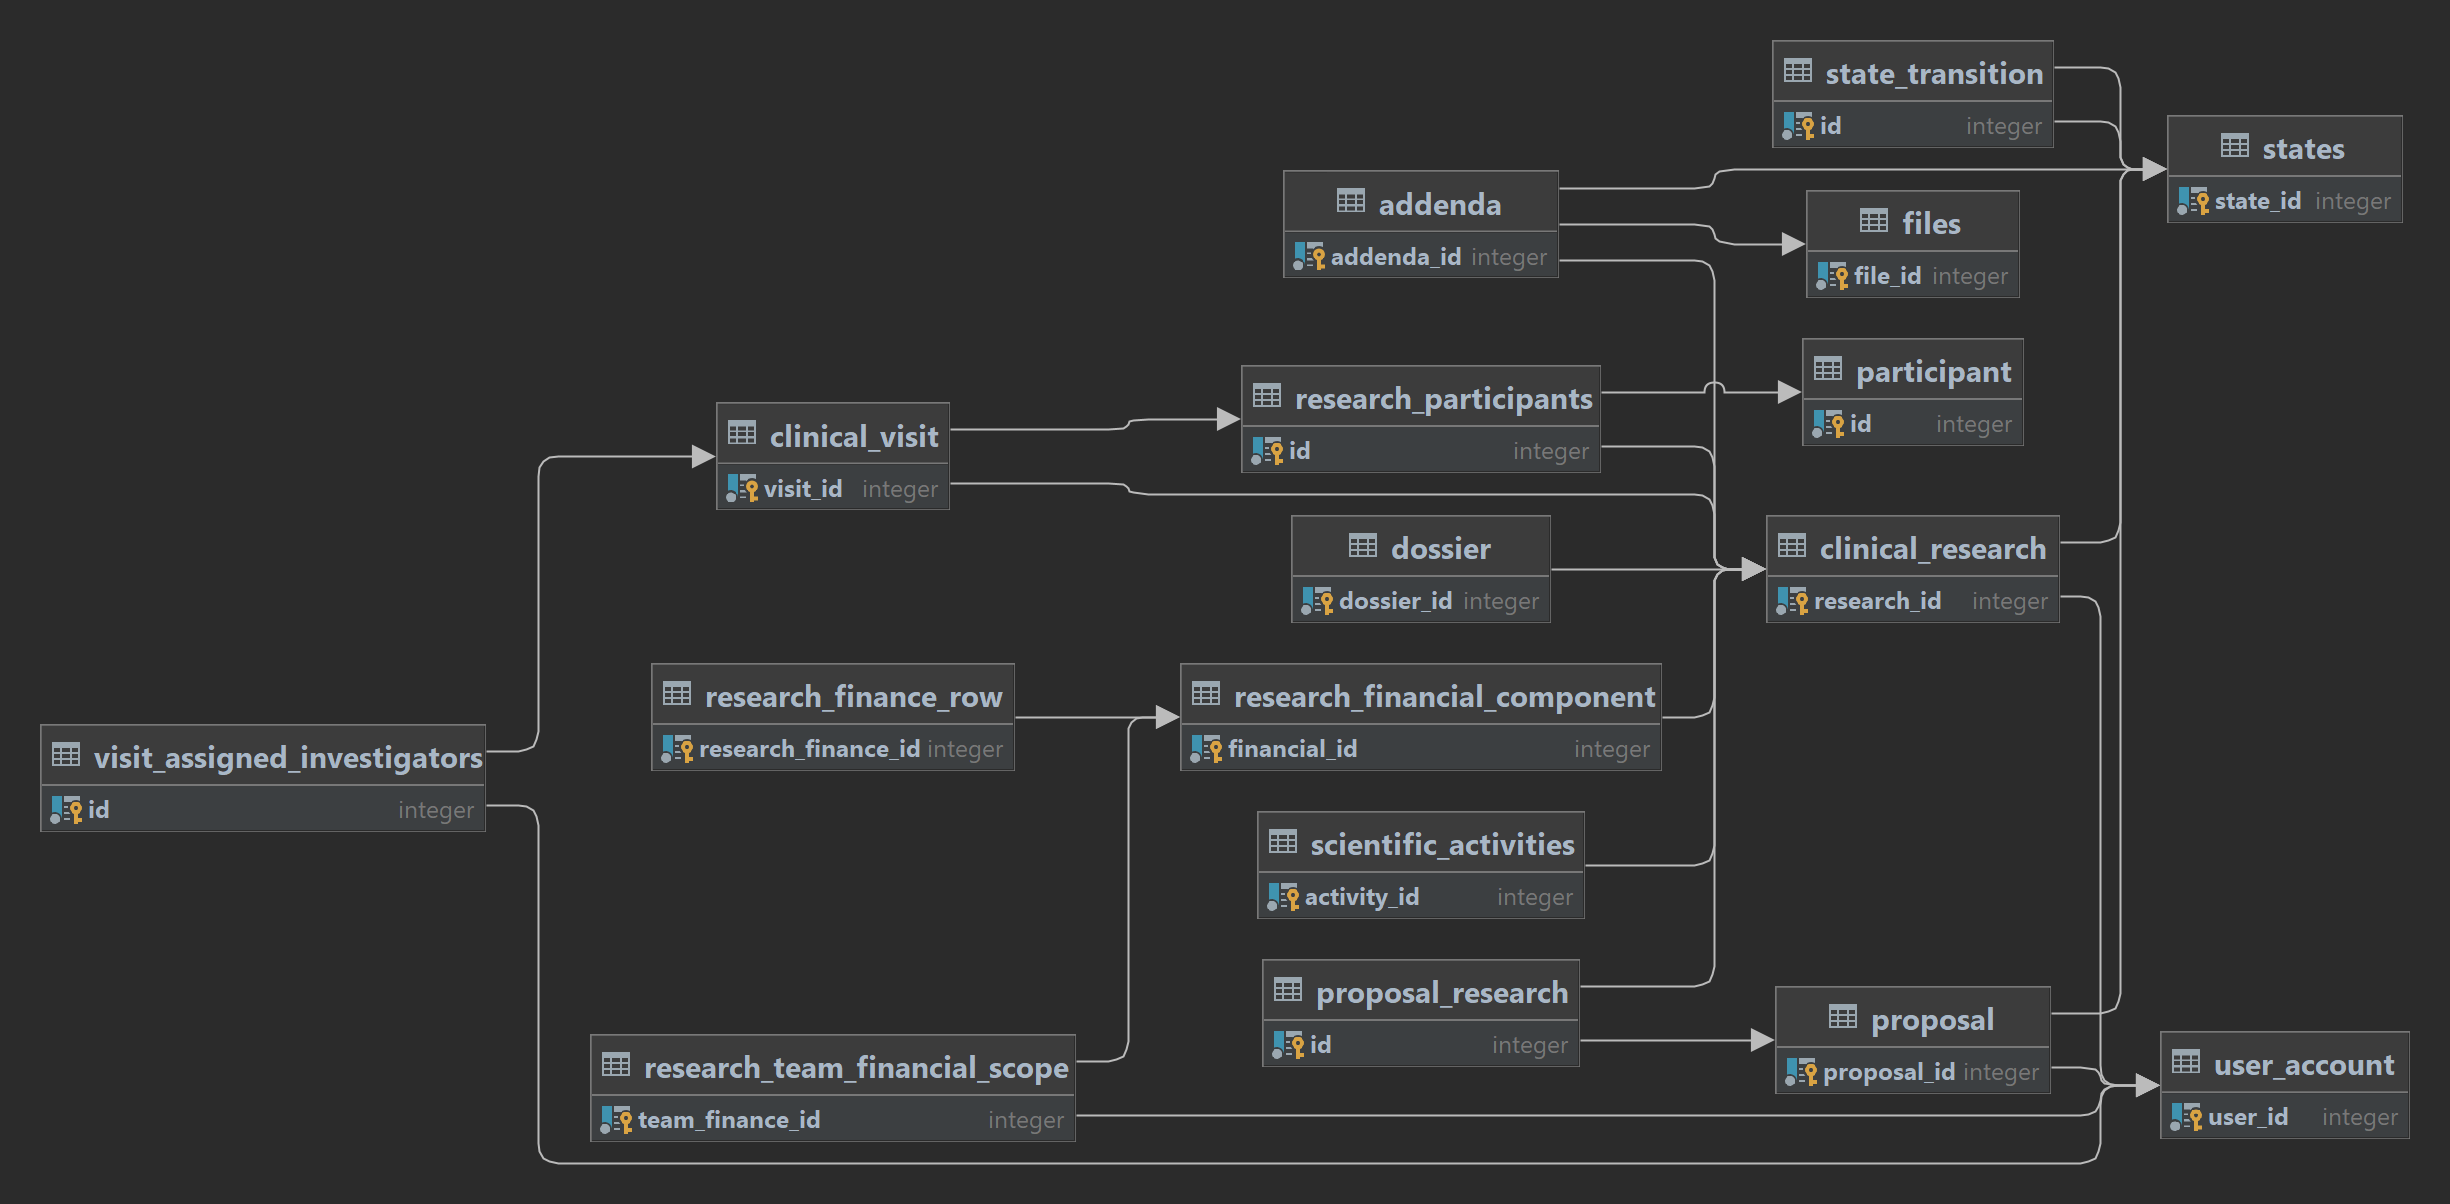
\includegraphics[scale=0.15]{Chapters/img/model/research-centered-er-diagram.png}
    \caption{Entity relationship diagram centered on the Clinical Research Entity.}
    \label{fig:er-diagram-research}
\end{figure}

